\PassOptionsToPackage{dvipsnames}{xcolor}
\documentclass[border=0mm]{standalone}
\usepackage[dvipsnames]{xcolor}
\usepackage{amsmath}
\usepackage{amssymb}
\usepackage{dsfont}
\usepackage{bm}
\usepackage{tikz}
\usetikzlibrary{arrows}
\usetikzlibrary{calc}
\usetikzlibrary{shapes}
\usepackage{upgreek}

\usepackage{esvect}
\newcommand{\cev}[1]{\reflectbox{\ensuremath{\vv{\reflectbox{\ensuremath{#1}}}}}}


\definecolor{color1}{rgb}{0,0.4470,0.7410}
\definecolor{color2}{rgb}{0.8500,0.3250,0.0980}
\definecolor{color3}{rgb}{0.9290,0.6940,0.1250}
\definecolor{color4}{rgb}{0.4940,0.1840,0.5560}
\definecolor{color5}{rgb}{0.4660,0.6740,0.1880}
\definecolor{lightblue}{RGB}{86,192,150}

\pgfdeclarelayer{background layer}
\pgfdeclarelayer{foreground layer}
\pgfsetlayers{background layer,main,foreground layer}


\begin{document}



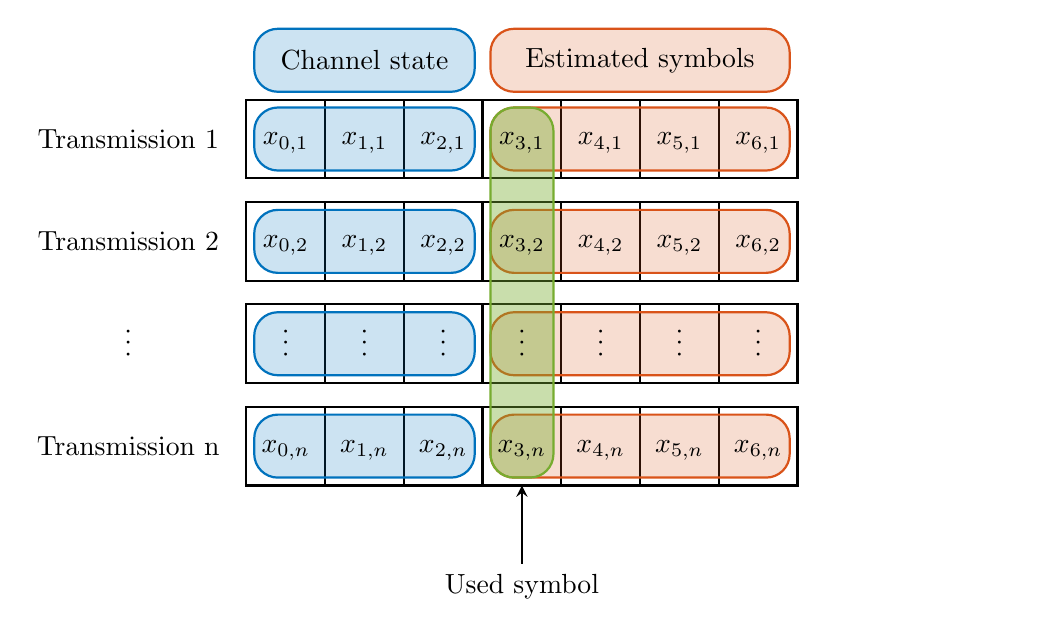
\begin{tikzpicture}[>=stealth,thick]

  \foreach \y in {1,...,4}{ 
    \foreach \x in {0,...,6}
    {
     \draw [thick] (\x,-\y-0.3*\y) +(-.5,-.5) rectangle ++(.5,.5);
     \begin{pgfonlayer}{foreground layer}
     \ifnum\y=3
      \draw (\x,-\y-0.3*\y) node [anchor=center]{$\cdot$};
      \draw (\x,-\y-0.35*\y) node [anchor=center]{$\cdot$};
      \draw (\x,-\y-0.25*\y) node [anchor=center]{$\cdot$};
      \else
     \ifnum\y=4
      \draw (\x,-\y-0.3*\y) node [anchor=mid]{$x_{\x,n}$};
      \else
      \draw (\x,-\y-0.3*\y) node [anchor=mid]{$x_{\x,\y}$};
       \fi
     \fi
     \end{pgfonlayer}
    }
    \ifnum\y=3
      \draw (-2,-\y-0.3*\y) node [anchor=center]{$\cdot$};
      \draw (-2,-\y-0.35*\y) node [anchor=center]{$\cdot$};
      \draw (-2,-\y-0.25*\y) node [anchor=center]{$\cdot$};
      \else
     \ifnum\y=4
    \node [] at (-2, -\y-0.3*\y) {Transmission n};
      \else
    \node [] at (-2, -\y-0.3*\y) {Transmission \y};
       \fi
      \fi
    \node [anchor=west] at (6.7, -\y-0.3*\y) {\phantom{Transmission \y}};
    \draw [thick,rounded corners =0.3cm, color1, fill=color1,fill opacity=0.2](0,-\y-0.3*\y) +(-.4,-.4) rectangle ++(2.4,.4);
    \draw [thick,rounded corners =0.3cm, color2, fill=color2,fill opacity=0.2](3,-\y-0.3*\y) +(-.4,-.4) rectangle ++(3.4,.4);
}

    \draw [thick,rounded corners =0.3cm, color5, fill=color5,fill opacity=0.4](3,-1.3) +(-.4,-4.3) rectangle ++(.4,.4);

    \draw [thick,rounded corners =0.3cm, color1, fill=color1,fill opacity=0.2](0,-0.3) +(-.4,-.4) rectangle ++(2.4,.4) node[black,pos=.5,opacity=1] {Channel state};
    \draw [thick,rounded corners =0.3cm, color2, fill=color2,fill opacity=0.2](3,-0.3) +(-.4,-.4) rectangle ++(3.4,.4)node[black,pos=.5,opacity=1] {Estimated symbols};

    \draw [<-,thick] (3,-5.7) --+ (0,-1) node [below]{Used symbol};

\end{tikzpicture}

\end{document}
























